\section{Background}
\label{sec:relwork}
Both Gramatron and Nautilus are built on top of American Fuzzy Lop (AFL), an instrumentation guided greybox fuzzing tool. Gramatron and Nautilus differs in their ways of mutating input testcases and are therefore potentially better suited for different tasks. 

\paragraph{American Fuzzy Lop.}
American Fuzzy Lop (AFL) is a greybox fuzzing tool. Unlike black box fuzzing, AFL is able to obtain the path coverage information of a particular seed (an AFL-generated test input) through instrumentation and decide whether to keep the seed by observing if a new program path is traversed. However, unlike white box fuzzing, the mutation from one seed to another is of random nature. A simplified version of AFL's work flow can be described as follows.
\begin{enumerate}
    \item AFL loads user provided seeds into its internal queue.
    \item Choose a seed from the queue to mutate. \label{itm:2}
    \item Mutate the seed using the mutation strategies available. \label{itm:3}
    \item If the new seed increases path coverage, AFL saves it to queue.
    \item Go to \ref{itm:2}.
\end{enumerate}

I used AFLplusplus, an extension of AFL, in this project \cite{257204}. AFLplusplus extends AFL by adding a custom mutator API, which makes it easier to use different mutation strategies in step \ref{itm:3}. In essence, Gramatron and Nautilus are different mutators that can be added on top of AFLplusplus. Gramatron and Nautilus only participate in step \ref{itm:3} of the fuzzing process. 

\paragraph{Nautilus.}
Nautilus is a grammar aware fuzzer that represents seed inputs as trees \cite{aschermann_frassetto_holz_jauernig_sadeghi_teuchert_2019}. \figref{nautilus-tree-representation} shows an example of such representation. With this internal data structure, Nautilus is able to perform a variety of tree mutations on the existing seeds to produce new seeds. Some of the tree mutations Nautilus can perform are listed below.
\begin{enumerate}
    \item Random Mutation. Nautilus picks a random node from the tree and replaces the subtree from the node with another randomly generated subtree.
    \item Random Recursive Mutation. Nautilus picks a recursive part of the tree and repeats it for up to $n$ times. \figref{nautilus-tree-representation-after-recursive-mutation} shows the result of applying random recursive mutation on the tree shown in \figref{nautilus-tree-representation}.
    \item Splicing Mutation. Nautilus combines two seeds from the queue by replacing a subtree from one seed with a subtree from another seed.
\end{enumerate}
\begin{figure}[h]
  \centering
  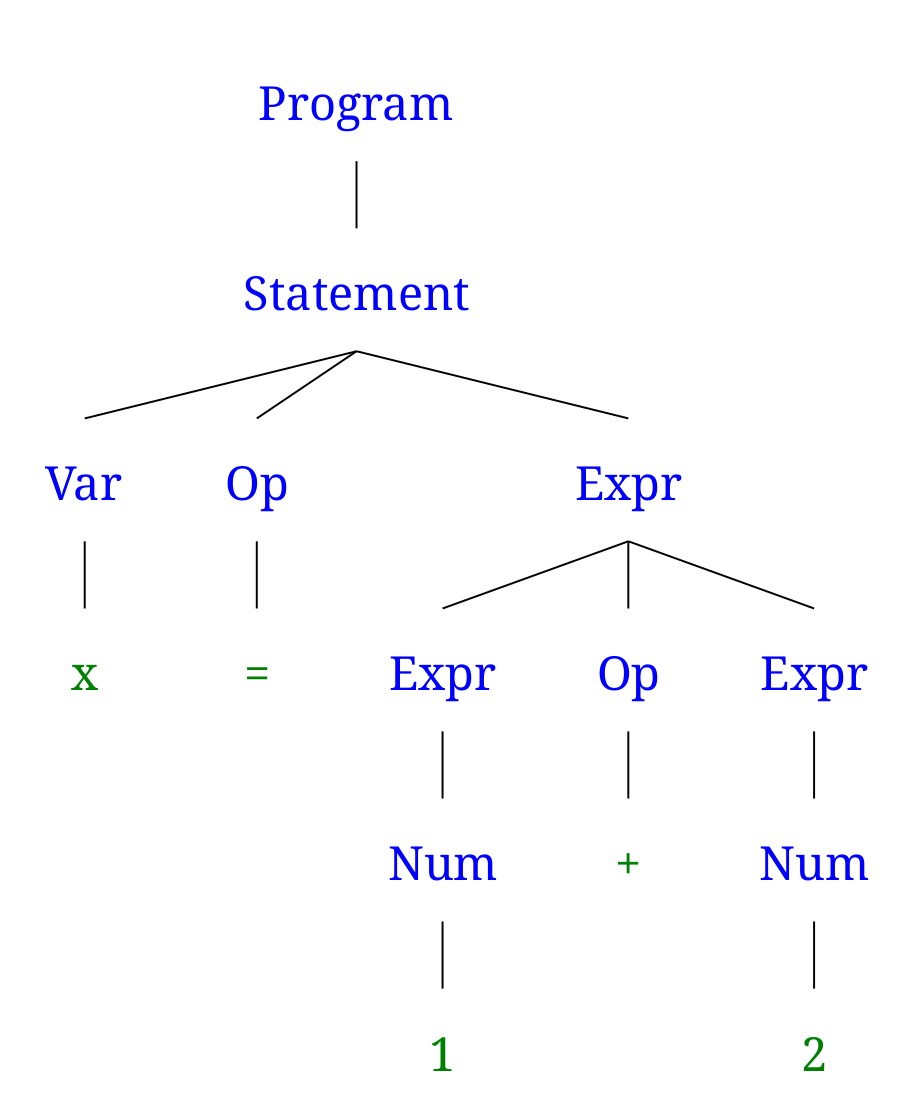
\includegraphics[scale=0.15]{images/parse-tree1.png}
  \caption{Nautilus Seed Representation. This tree represents input seed \texttt{x=1+2}.}\label{nautilus-tree-representation}
\end{figure}
\begin{figure}[h]
  \centering
  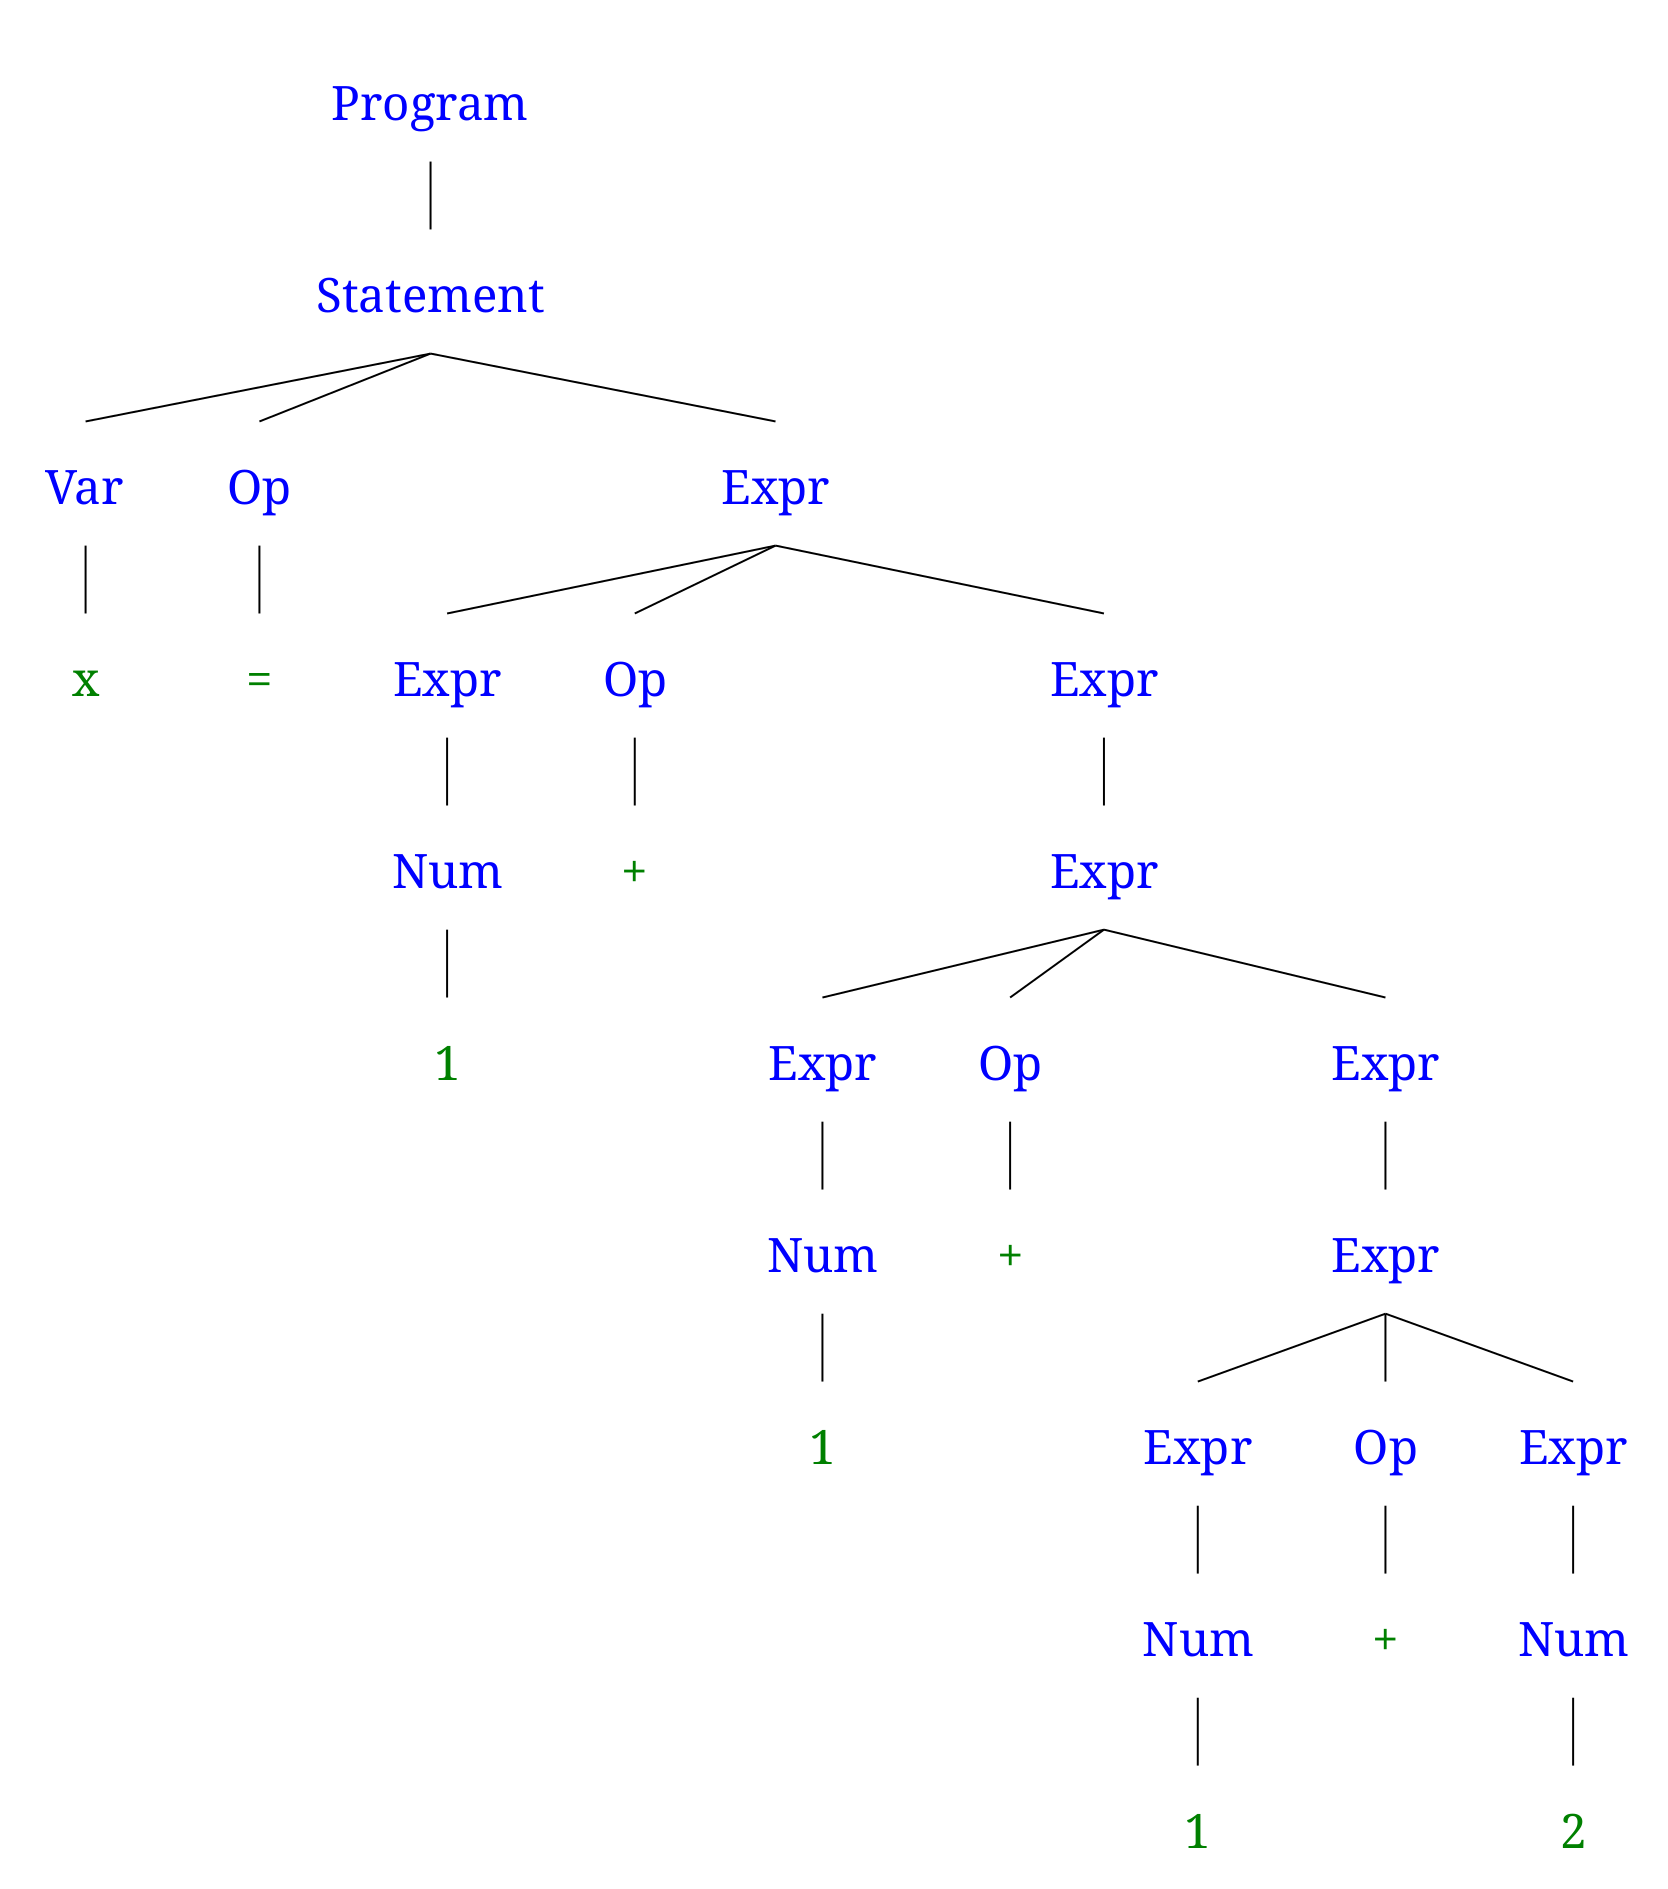
\includegraphics[scale=0.15]{images/parse-tree2.png}
  \caption{Nautilus Random Recursive Mutation. This tree represents the result of recursive mutation from \texttt{x=1+2} to \texttt{x=1+(1+(1+2))}.}\label{nautilus-tree-representation-after-recursive-mutation}
\end{figure}
One important characteristic of Nautilus is that its mutation are often localized. The overhead of making complex changes is big since it requires traversing down the tree to find the right node to mutate. It is also expensive to generate a new tree. Therefore, most of Nautilus' mutations only modify a subtree of the original seed. 

Nautilus has built-in function that can convert an input into tree representation. Therefore, Nautilus can accept user defined seeds.

\paragraph{Gramatron.}
Gramatron is a grammar aware fuzzer that represents the seed inputs as automaton walks \cite{srivastava_payer_2021}. Internally, it converts the input grammar into a finite state automaton (FSA). \figref{example-fsa} shows a subset of PHP grammar as a FSA. For example, \texttt{<?php rand(); ?>} can be represented by automaton walk $[0-1, 1-1, 2-1, 3-1]$.
\begin{figure}[h]
  \centering
  
\includegraphics[scale=0.35]{images/fsa.png}
  \caption{Finite State Automaton. This FSA represents a subset of PHP grammar. The indices in the square brackets represent the edges (state transitions) in the graph.}\label{example-fsa}
\end{figure}

Gramatron can perform three kinds of automaton-based mutation.
\begin{enumerate}
    \item Splice. Gramatron replaces part of a seed input's automaton walk with a subwalk from another seed.
    \item Random Mutation. Gramatron chooses a mutation point from the seed's automaton walk, discards the subwalk from that point and starts taking a random walk on the FSA to generate a new subwalk for the seed.
    \item Random Recursion. Gramatron replicates parts of the automaton walk that have recursive features up to $n$ times.
\end{enumerate}

Given an input seed and a point of mutation, Gramatron mutates until the end of the string. The overhead for performing this kind of mutation is smaller using automata than trees since the input is represented by a simple array using automata. This characteristic makes Gramatron's mutation more aggressive than Nautilus'. 

The current implementation of Gramatron does not include function that can parse an input into an automaton walk. Gramatron generates its own input seeds by walking the FSA randomly at the beginning. In this project, I implemented an automaton parser which enables Gramatron to use seeds generated by other mutators.
% Here is how you cite papers. For example, we read papers in the
% class~\cite{rahul2016pwtypos,dodisetal:2004}.  And here is some random citation~\cite{Bojinov:2010:KLP,schechter:2010:pen,everspaugh2015pythia,bellare2009format,Juels:2014}


% \subsection{Overview of the design}
% \label{sec:overview}

% And then just to showoff some \LaTeX skills, here is a Tikz plot.
% % \section{Diagrammatic view of Multisketch operations}\label{app:mainflow}  

% A user registers with a user id $\u$ and a vector of biometric templates
% $\mvec=\mvecss{\mlen}$. Multisketch uses two databases $\dbid$ and $\dbmsg$\@,
% where $\dbid$ contains user id $\u$ and the corresponding helper data
% $\sketchval$, and $\dbmsg$ contains the random permutation of the templates
% registered so far. Highlighted are the entries corresponding to a user $\u_4$
% with templates $\mvec_4=\mvec_{41}\ldots\mvec_{4\mlen}$.% and helper
%     % data $\sketchval_4$.
\begin{figure}[t]
  \centering
  \begin{tikzpicture}[
    >=stealth,
    node distance=2cm,
    database/.style={
      cylinder,
      cylinder uses custom fill,
      cylinder body fill=black!25!white,
      cylinder end fill=black!25!white,
      shape border rotate=90,
      aspect=0.25,
      minimum width=2em,
      minimum height=2em,
      draw
    },
    func/.style={
      rectangle,
      fill=red!25!white,
      minimum width=1cm,
      minimum height=1em,
      draw
    },
    cell/.style={
      rectangle,
      draw=black!50!white
    }
    ]
    \node (user) at (0, 0) {User};
    \node[func, right of=user, right=-1.1em, above=3em] (msketch) {$\MS$}; 
    \draw[below of=msketch, dashed, anchor=west] (.85,0.55) rectangle (5.9,-1.2); 
    \node[func, below of=msketch, anchor=east, below=1.95cm,fill=red!10!white,dashed] (mrecover) {$\MRec$};
    % \node[database, right of=user, anchor=south, above=1em, right=2cm] (db1) {$\dbid$};
    \matrix (db1) [right of=user, anchor=south, below=2pt, right=-0.1cm, 
    matrix of math nodes,
    column sep = -\pgflinewidth,
    row sep=-\pgflinewidth,
    column 1/.style={nodes={cell}}, 
    column 2/.style={nodes={cell}}, 
    anchor=west] {
      \u_1 & \sketchval_1\\
      \u_2 & \sketchval_2\\
      \u_3 & \sketchval_3\\
      |[draw,fill=blue!20]|\u_4 & |[draw,fill=blue!20]|\sketchval_4\\
    };
    \node[left of=db1, anchor=east,right=1.1cm] {$\dbid$};
    \matrix (db2) [right of=db1, left=25pt, matrix of math nodes,
    column sep = 2\pgflinewidth,
    row sep=-\pgflinewidth,
    column 1/.style={nodes={cell}},
    column 2/.style={nodes={cell}}, 
    column 3/.style={nodes={cell}}, 
    column 4/.style={nodes={cell}}, 
    column 5/.style={nodes={cell}}, 
    anchor=west] {
      \mvec_{21} &\mvec_{12} & |[draw,fill=blue!20]|\mvec_{43} &  & \mvec_{3\mlen} \\
      |[draw,fill=blue!20]|\mvec_{41} &\mvec_{32} & \mvec_{33} & |[draw=white]|\ldots & \mvec_{2\mlen} \\
      \mvec_{11} &|[draw,fill=blue!20]|\mvec_{42} & \mvec_{23} &  & \mvec_{1\mlen} \\
      \mvec_{31} &\mvec_{22} & \mvec_{13} & & |[draw,fill=blue!20]|\mvec_{4\mlen} \\
    };
    \node[left of=db2, left=-4pt] {$\dbmsg$};

    % \node[database,right of=db1] (db2) {$\dbmsg$};
    \node[func,below of=db1,anchor=north,above=8pt,left=8pt] (gu) {GetUser};
    \node[func,right of=gu,anchor=east,right=-5pt] (fm) {FindMatches};
    \node[func,below of=db1,anchor=east,below=2em,right=-3pt] (recover) {Recover};

    \draw[->,blue!50,thick] (user.north) |- node[black,near end,above]{$u, \mvec$} node[black,near end,below,font=\small]{register} 
    (msketch.west);
    \draw[->,blue!50,thick] (msketch) -| node[black,near end, left,right]{$u, \sketchval$} (db1);
    \draw[->,blue!50,thick] (msketch) -| node[black,near end, left,right]{$\mvec$} (db2);

    \draw[->,blue!50,thick] (user.south) |- ++(1,-0.9) node[black,near end,above]{$u, \mvectilde$} node[black,near end,below,font=\small]{login}   -| node[black,left,near end]{$u$}
    (gu.north);
    \draw[->,blue!50,thick] (user.south) |- ++(0,-0.9)  -- ++(3.1,0) |- node[black,near end, above]{$\mvectilde$}
    (fm.west);
    \draw[->,blue!50,thick] (db1.south) |- node[black,near end,above]{} (gu.east);
    \draw[->,blue!50,thick] (db2.south) |- node[black,near end,above]{} (fm.east);
    \draw[->,blue!50,thick] (gu.south) |- node[black,near end,above]{$\sketchval$} (recover.west);
    \draw[->,blue!50,thick] (fm.south) |- node[black,near end,above]{$\mvec'$} (recover.east);    
    \draw[->,blue!50,line width=2pt] (recover.south) -- node[black,near end,right]{$\mvec$ or $\bot$} ++(0, -0.65);
  \end{tikzpicture}
  % \rcnote{Rough sketch of the flow of the \biosketch.} 
  \caption{Diagram of multisketch as a part of an authentication service. 
  }
  \label{fig:mainflow}
\end{figure}

%%% Local Variables:
%%% mode: latex
%%% TeX-master: "../main"
%%% End:


% You refer to a figure in the following way. In~\figref{fig:mainflow} we show
% some thing that is relevant for the Multisketch paper by Chatterjee et
% al.~\cite{chatterjee2019multisketches}. Add your bibliography to the
% \textsf{bib.bib} file. You can copy the Bibtex format citation from Google
% Scholar.
